\chapter{Implementation Model}

Figure \ref{implementation_model} shows the architecture of a typical, multi-threaded
implementation. It includes two processes dedicated to each server,
a peer process to receive messages from the server or reference
clock, and a poll process to transmit messages to the server or
reference clock.

\begin{figure}
\centering
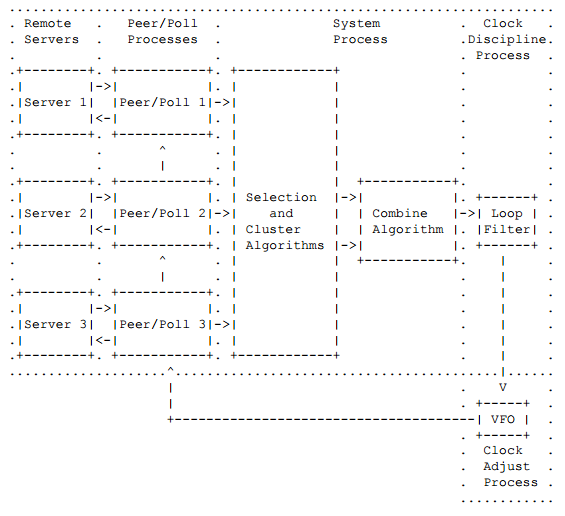
\includegraphics[width=\textwidth]{implementation_model.png}
\caption{Implementation Model}
\label{implementation_model}
\end{figure}

These processes operate on a common data structure, called an
association, which contains the statistics described above along with
various other data described in Section 9. A client sends packets to
one or more servers and then processes returned packets when they are
received. The server interchanges source and destination addresses
and ports, overwrites certain fields in the packet and returns it
immediately (in the client/server mode) or at some time later (in the
symmetric modes). As each NTP message is received, the offset theta
between the peer clock and the system clock is computed along with
the associated statistics delta, epsilon, and psi.

The system process includes the selection, cluster, and combine
algorithms that mitigate among the various servers and reference
clocks to determine the most accurate and reliable candidates to
synchronize the system clock. The selection algorithm uses Byzantine
fault detection principles to discard the presumably incorrect
candidates called ``falsetickers'' from the incident population,
leaving only good candidates called ``truechimers''. A truechimer is a
clock that maintains timekeeping accuracy to a previously published
and trusted standard, while a falseticker is a clock that shows
misleading or inconsistent time. The cluster algorithm uses
statistical principles to find the most accurate set of truechimers.
The combine algorithm computes the final clock offset by
statistically averaging the surviving truechimers.

The clock discipline process is a system process that controls the
time and frequency of the system clock, here represented as a
variable frequency oscillator (VFO). Timestamps struck from the VFO
close the feedback loop that maintains the system clock time.
Associated with the clock discipline process is the clock-adjust
process, which runs once each second to inject a computed time offset
and maintain constant frequency. The RMS average of past time offset
differences represents the nominal error or system clock jitter. The
RMS average of past frequency offset differences represents the
oscillator frequency stability or frequency wander. These terms are
given precise interpretation in Section 11.3.

A client sends messages to each server with a poll interval of $ 2^\tau $
seconds, as determined by the poll exponent tau. In NTPv4, tau
ranges from 4 (16 s) to 17 (36 h). The value of tau is determined by
the clock discipline algorithm to match the loop-time constant $ T_c = 2^\tau $.
In client/server mode, the server responds immediately;
however, in symmetric modes, each of two peers manages tau as a
function of current system offset and system jitter, so they may not
agree with the same value. It is important that the dynamic behavior
of the clock discipline algorithm be carefully controlled in order to
maintain stability in the NTP subnet at large. This requires that
the peers agree on a common tau equal to the minimum poll exponent of
both peers. The NTP protocol includes provisions to properly
negotiate this value.

The implementation model includes some means to set and adjust the
system clock. The operating system is assumed to provide two
functions: one to set the time directly, for example, the Unix
settimeofday() function, and another to adjust the time in small
increments advancing or retarding the time by a designated amount,
for example, the Unix adjtime() function. In this and following
references, parentheses following a name indicate reference to a
function rather than a simple variable. In the intended design the
clock discipline process uses the adjtime() function if the
adjustment is less than a designated threshold, and the
settimeofday() function if above the threshold. The manner in which
this is done and the value of the threshold as described in
Section 10.
